\documentclass{article}
\usepackage{setspace}
\doublespacing

%MarginHar staten k\o bt verdens dyreste forsikring af Goldman Sachs
\usepackage{geometry}
\geometry{left=2.5cm,top=2.5cm,right=2.5cm,bottom=2.5cm}

%Dansk opsaetning
%\usepackage[apalike]{dk-bib}
\usepackage[utf8]{inputenc} 
\usepackage[danish]{babel} 
\renewcommand{\danishhyphenmins}{22} 
\usepackage[T1]{fontenc}
\usepackage{amsmath, mathtools, natbib, graphicx, placeins, tabularx,booktabs, tikz, pdflscape}
\usetikzlibrary{calc}
%\usepackage[. . .]{endfloat}

\usepackage[danish=quotes]{csquotes}

\usepackage{titlesec}
\usepackage[titletoc,toc,title]{appendix}

\title{En Ex-Ante Evaluering af DONG Aftalen\thanks{Vi er taknemmelige for kommentarer fra Hannes Malmberg, Hans Henrik Sievertsen, Andreas Noack, Robin Brejnholt, Erik {\"O}berg, Kasper Harbo Hansen, Line Elvstrøm Ekner, Jon Kjellund,  Jens Houe Thomsen, Brian Thuesen samt deltagere ved EPRU et seminar i København. Alle udestående fejl er naturligvis vores egne.  Programmer og data er tilgængelige på \texttt{https://github.com/njharbo/DONG}.} \\ }
%\emph{Working paper}
%Christian Stassen,
\author{Niels-Jakob Harbo Hansen\thanks{Korresponderende forfatter. Stockholm University, IIES.  Email: \texttt{nielsjakobharbo.hansen@iies.su.se}. Niels-Jakob er PhD studerende i nationaløkonomi ved IIES i Stockholm.} \hspace{0.1 mm} og Guan Yang\thanks{Email: \texttt{guan@yang.dk} Guan er PhD i Finansiering fra New York University.  }. }


\begin{document}

\maketitle

\begin{abstract}
\onehalfspacing
 Vi evaluerer 2014-aftalen om DONG Energy imellem stat og private investorer imod et alternativ hvor staten selv indskød ny aktiekapital i DONG. Målt imod dette alternativ er den indgåede aftale stærkt asymmetrisk: staten afskrev sig mulighed for gevinst i scenarier med en positiv udvikling i DONGs værdi, men betalte stadig en stor del af tabet i negative scenarier. I vores simulationer er det forventede tab på aftalen [1.6; 4.1] mia. DKK jævnført med alternativet. Samtidig viser vi, at den indbyggede put-option i aftalen betød, at de private investorer reelt betalte væsentligt under de oplyste 107.25 DKK per aktie. \\
 JEL-codes: G32, G34 \\
 Key-words: Capital Injection, Firm Ownership
\end{abstract}


\newpage

\section{Introduktion}

%TBD: CHANGE CALCULATION FORMULAR. ADD VARIATION IN INITIAL MARKET PRICE IN MAIN TEXT. FIGURE CHECK. LAES AKTSTYKKE. SKRIV OM ATP ROLLE I SPILTRAE. KLARGOER AT VI BYGGER PÅ TILGAENGELIG INFO.

I januar 2014 vedtog Folketingets finansudvalg en aftale om udvidelse af aktiekapitalen i DONG Energy A/S. Med aftalen mellem staten, det Goldman Sachs-forvaltede investeringsselskab New Energy Investment og de to danske pensionskasser ATP og PFA opnåede DONG et kapitalindskud på 11 mia. DKK.\footnote{Dertil kom op til 2.6 mia. DKK fra eksisterende mindretalsaktionærer, hvilket vi dog vil se bort fra i analysen nedenfor.} I forbindelse med salget skrev vi den 27. januar 2014 en kommentar om salget i Dagbladet Information \citep{Hansen2014}. Denne artikel under- og udbygger disse beregninger.

I artiklen stiller vi spørgsmålet: \emph{Var aftalen økonomisk set bedre end et alternativt hvor staten selv skød aktiekapital ind i DONG?} Konkret etablerer vi en beregningsstruktur som gør det muligt kvantitativt, at evaluere den indgåede aftale mod et alternativ, hvor staten selv skød kapital ind i DONG og finansierede dette igennem udstedelse af statsobligationer. Vi viser først, at afkaststrukturen i den indgåede aftale er stærkt asymmetrisk sammenlignet med det offentlige alternativ på grund af den put-option som er indbygget i den indgåede aftale. Specifikt opnår staten en gevinst på aftalen, sammenlignet med det offentlige alternativ, hvis værdien af DONG gennemsnitligt falder med mere end 3.6\% per år frem mod 2018. Imidlertid er den gevinst, som staten opnår, hvis DONGs værdi udvikler sig negativt, begrænset i forhold til\ det tab, staten får i scenarier, når DONGs værdi udvikler sig positivt. Det vil sige, at staten med aftalen hovedsageligt har \enquote{forsikret} sig mod at opnå et positivt afkast. 

For at beregne statens forventede afkast på aftalen, sammenlignet med det offentlige alternativ, er to spørgsmål afgørende. For det første, hvad var den reale markedspris for DONGs egenkapital i starten af 2014? For det andet, hvad er sandsynlighedsfordelingen på væksten i DONGs værdi frem mod 2018? 

I vores benchmark-beregninger antager vi, at DONGs initiale markedspris lå i intervallet 24-38 mia. sådan som DONG selv har anslået. Desuden antager vi, at den fremtidige vækst i DONGs værdi trækkes fra den historiske afkastfordeling fra europæiske elektricitetsselskaber. Med disse antagelser er det forventede tab på aftalen jævnført med et offentligt alternativ i intervallet [1.6; 4.1] mia. DKK. Sandsynligheden for at den indgåede aftale giver et bedre afkast end det offentlige alternativ er cirka 50\%, men qua den asymmetriske afkaststruktur, hvor staten tager en del af downside, men ikke får nogen upside, opvejer det bedre afkast, i scenarier hvor værdien af DONGs egenkapital falder, ikke det afkast staten går glip af i  scenarier, hvor DONGs egenkapital stiger i værdi.

%markedspris reelt var 107.25 DKK per aktie (totalt 31.5 mia.DKK) i 2014, og altså lig med den pris som  Finansministeriet og DONG har udtalt at DONG's egenkapital blev handlet til. Desuden antager vi, at den fremtidige vækst i DONGs værdi trækkes fra den historiske afkastfordeling fra europæiske elektricitetsselskaber. Med disse antagelser bliver det forventede tab på aftalen på ca.\ 2.5 mia.\ DKK. Sandsynligheden for at den indgåede aftale giver et bedre afkast end det offentlige alternativ er cirka 50\%, men qua den asymmetriske afkaststruktur, hvor staten tager en del af downside, men ikke får nogen upside, opvejer det bedre afkast, i scenarier hvor værdien af DONGs egenkapital falder, ikke det afkast staten går glip af i  scenarier, hvor DONGs egenkapital stiger i værdi.

En vigtig pointe er dog, at de private investorer reelt \emph{ikke} betalte 107.25 DKK per aktie for DONGs egenkapital, svarende til initial værdi af DONGs egenkapital på 31.5 mia. DKK som oplyst i  \cite{FM2013a}. De 107.25 DKK afspejlede prisen for en portefølje bestående af \emph{både} DONGs egenkapital \emph{og} en put-option. For at finde den pris de private investorer reelt betalte for DONGs egenkapital, er det nødvendigt at korrigere de 107.25 DKK for prisen på put-optionen. I vores beregninger, finder vi at de private investorer kun betalte den faktiske markedsværdi for DONG hvis denne primo 2014 var 24.5 mia. DKK. Hvis DONGs markedsværdi primo 2014 reelt var 31.5 mia. DKK, så finder vi at selskabet reelt handlet for 27.2 mia. DKK.

Det er vigtigt at understrege, at der en række usikkerhedsmomenter i disse beregninger. Dette drejer sig om 1) valget af afkastfordeling, 2) fastsættelse af DONGs initiale værdi og 3) valget af volatilitet i beregningen af put-optionens værdi. Vi undersøger derfor beregningernes robusthed i forhold til disse antagelser i vores appendix.

Vi er ikke de første, der har undersøgt DONG aftalen. \cite{Bachman2014} analyserer aftalen og de argumenter der har været fremført for og imod salget. Forfatterne konkluderer, at mange af de brugte argumenter imod aftalen har været præget af misforståelser, men forfatterne har også svært ved at se formålet ved den transaktion, som staten valgte i forhold til en mere simpel kapitaludvidelse hvor private investorer, og eventuelt staten, indskød den kapital DONG manglede. Vi komplementerer artiklen af \cite{Bachman2014} ved, at begå en \emph{kvantitativ} evaluering af den indgåede aftale i forhold til et offentligt alternativ. 

Resten af artiklen er opbygget som følger; I afsnit 1 gennemgår vi kort aftalen fra 2014. I afsnit 2 vurderer vi aftalen overfor et offentligt alternativ, og i afsnit 3 konkluderer vi.


\section{Aftalen}
I efteråret 2013 indgik staten en aftale med et konsortium af private investorer om en aktieudvidelse i DONG Energy A/S på 11 mia.\ DKK.\footnote{Dette afsnit bygger på \citet{FM2013a}.} Specifikt indskød det Goldman Sachs-kontrollerede selskab New Energy Investment (NEI) 8 mia.\ DKK, mens de to danske pensionskasser, ATP og PFA, samlet indskød 3 mia.\ DKK.\footnote{Dertil kom op til 2.6 mia.\ DKK yderligere fra eksisterende mindretalsaktionærer, hvilket vi dog vil se bort fra i analysen nedenfor.}

Aftalen var en kapitaludvidelse, men samtidigt tildelte staten de nye aktionærer en salgsret (en put-option), som under visse omstændigheder giver investorerne ret til, at sælge deres aktier tilbage til staten. Konkret giver salgsretten de private investorer retten til, at sælge deres aktier tilbage til staten,  til enten (i) markedsprisen,\footnote{Da aktierne i dette tilfælde ikke vil blive handlet på et marked så bestemmes markedsprisen af en tredje part.} eller (ii) markedsprisen for 40\% af aktierne og 60\% af aktierne forrentet med den årlige Cita-rente, baseret på rentekurven ultimo 2013, tillagt 2.25\%.\footnote{I \citet{FM2013f} er Cita-renten oplyst til, at være 0.13\%, 0.44\%, 0.88\% og 1.46\% i 2014--17. Forretningen er baseret på Cita-kurven på det tidspunkt hvor aftalen blev indgået, og afspejler altså ikke den efterfølgende udvikling i renteniveauet.}

Hvorvidt salgsretten kan udnyttes, afhænger af status for børsnoteringen af DONG og perioden. Periode 1 løber til og med den 45. dag efter offentliggørelsen af årsregnskabet for 2017, mens periode 2 efterfølgende løber til ultimo 2020. Staten og de private investorerer er enige om, at arbejde mod en børsnotering af DONG inden 2018. Men hvis ikke DONG børsnoteres inden udløbet af periode 1, så får de private investorer ret til at udnytte deres salgsret, så længe dette sker, inden en børsnotering er igangsat.\footnote{Hvis salgsretten udnyttes i en situation hvor staten har igangsat en børsnotering, afregnes 60\% af aktierne til  forrentet med den årlige Cita-rente tillagt 2.25\%, men 40\% af aktierne overdrages til staten uden beregning.} Frem til slutningen af periode 1 har både NEI og staten ret til at vedlægge veto mod en børsnotering.\footnote{Endvidere skal ATP give deres samtykke, såfremt den forventede værdi af DONG Energy ligger under et givent, ej oplyst, niveau.} Efter denne dato kan staten alene beslutte at igangsætte en børsnotering.

En rimelig antagelse er derfor, at de private investorer udnytter salgsretten primo 2018 hvis de på dette tidspunkt vurderer markedsværdien af DONG til, at være mindre end den pris, som staten har forpligtet sig til at købe aktierne tilbage til. Vi kan indse dette gennem baglæns induktion af spiltræerne i Figur \ref{fig:tree_1} og \ref{fig:tree_2}. Vi gør dette i detaljer i Appendix \ref{sec:app_tree}, men kort sagt er argumentet:

\begin{itemize}
	\item Hvis markedsprisen i periode 2 ligger under prisen specificeret i salgsretten, har staten incitament til at starte børsnoteringen, mens de private investorer har incitament til, at udnytte salgsretten før dette sker. Resultatet vil her være, at de private investorer udnytter salgsretten eller, at staten egenhændigt igangsætter en børsnotering.\footnote{Hvorvidt staten i dette scenarie virkelig kan igangsætte en børsnotering før investorerne udnytter deres salgsret er imidlertid tvivlsomt. Dette vil kræve at staten egenhændigt starter en børsnotering uden de øvrige ejeres vidende.}
	\item Hvis markedsprisen i periode 2 ligger over prisen i salgsretten, så har de private investorer ikke incitament til at udnytte salgsretten. Resultatet vil her være en børsnotering, eller at staten overtager investorernes aktier til markedspris.
	\item Ved indgangen til periode 2 har de private investorer således incitament til, at udnytte salgsretten hvis markedsprisen ligger under prisen specificeret i salgsretten (strikeprisen), idet de hermed sikrer at staten ikke egenhændigt igangsætter en børsnotering, hvormed de private investorer mister retten til at sælge 60\% af aktierne forrentet med Cita-renten plus 2.25\% og 40\% af aktierne til markedspris.
\end{itemize} 

\begin{figure}
\includegraphics[scale=0.6]{../figs/perioder}
\caption{Illustration af perioder i statens aftale med de private investorer. Kilde: \citet{FM2013a}}
\label{fig:perioder}
\end{figure}

\begin{landscape}
\begin{figure}
\label{fig:tree_1}
\caption[]{Spiltræ hvis aktiepris $>$ garanteret tilbagekøbspris. I hver tom node tager staten en beslutning. I hver fyldt node tager NEI en beslutning. En firkantet node er blot et forbindelsespunkt.}
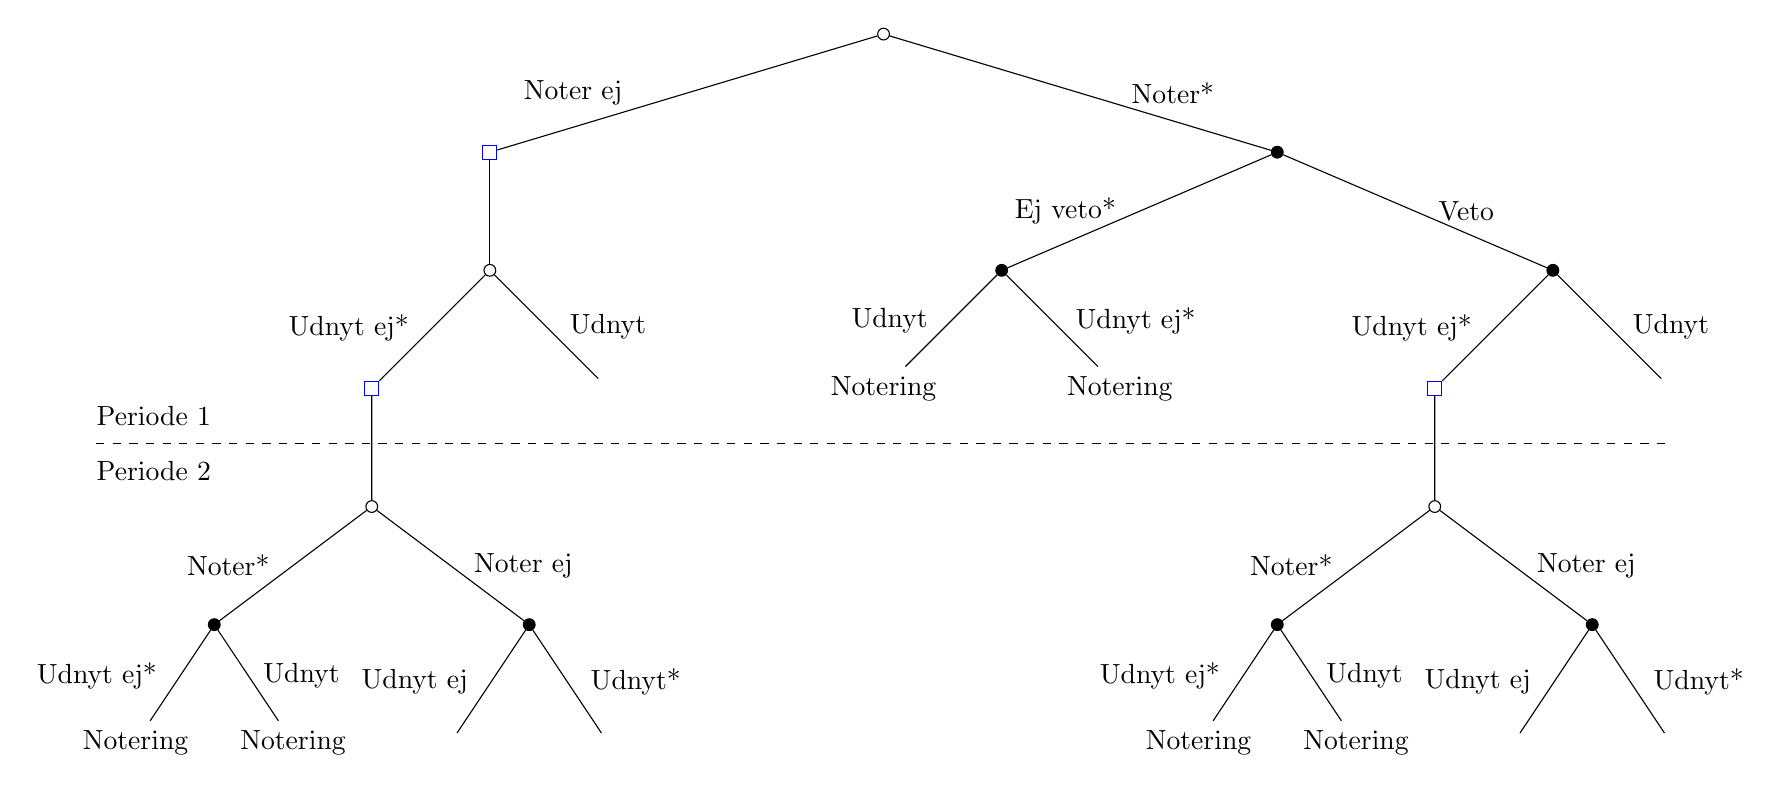
\begin{tikzpicture}
% Specify spacing for each level of the tree
\tikzstyle{level 1}=[level distance=15mm,sibling distance=100mm]
\tikzstyle{level 2}=[level distance=15mm,sibling distance=70mm]
\tikzstyle{level 3}=[level distance=15mm,sibling distance=30mm]
\tikzstyle{level 4}=[level distance=15mm,sibling distance=20mm]
\tikzstyle{level 5}=[level distance=15mm,sibling distance=40mm]
\tikzstyle{level 6}=[level distance=15mm,sibling distance=20mm]
\tikzstyle{hollow node}=[circle,draw,inner sep=1.5]
\tikzstyle{solid node}=[circle,draw,inner sep=1.5,fill=black]
\tikzset{
red node/.style={circle,draw=red,inner sep=1.2},
blue node/.style={rectangle,draw=blue,inner sep=2.5}
}
\node[hollow node]{}
child{node[blue node]{} 
child{node[hollow node]{}
child{node[blue node]{}  
child{node[hollow node]{}
child{node[solid node]{} 
child{node[]{Notering} edge from parent node[left,xshift=-5]{Udnyt ej*} } 
child{node[]{Notering} edge from parent node[right,xshift=2]{Udnyt} }
edge from parent node[left,xshift=-5]{Noter*} 
}
child{node[solid node]{} 
child{node[]{} edge from parent node[left,xshift=-5]{Udnyt ej} } 
child{node[]{} edge from parent node[right,xshift=5]{Udnyt*} }
edge from parent node[right,xshift=5]{Noter ej} 
}
}
edge from parent node[left,xshift=-5]{Udnyt ej*}
} 
child{node[]{} edge from parent[] node[right,xshift=5]{Udnyt} } 
}
edge from parent node[left,xshift=-20]{Noter ej}
}
child{node[solid node]{} 
child{node[solid node]{} 
child{node[]{Notering} edge from parent[] node[left,xshift=-5]{Udnyt} }
child{node[]{Notering} edge from parent[] node[right,xshift=5]{Udnyt ej*} }
edge from parent[] node[left,xshift=-5]{Ej veto*} }
child{node[solid node]{} 
child{node[blue node]{}  %Extended
child{node[hollow node]{}  
child{node[solid node]{} 
child{node[]{Notering} edge from parent[] node[left,xshift=-5]{Udnyt ej*} } 
child{node[]{Notering} edge from parent[] node[right,xshift=2]{Udnyt} }
edge from parent node[left,xshift=-5]{Noter*}  
}
child{node[solid node]{}  
child{node[]{} edge from parent[] node[left,xshift=-5]{Udnyt ej} } 
child{node[]{} edge from parent[] node[right,xshift=5]{Udnyt*} }
edge from parent[thin] node[right,xshift=5]{Noter ej} 
}
}
edge from parent[] node[left,xshift=-5]{Udnyt ej*}
}
child{node[]{} edge from parent node[right,xshift=5]{Udnyt} }
edge from parent[thin] node[right,xshift=5]{Veto} 
}
edge from parent[] node[right,xshift=15]{Noter*}
}
%child{node[blue node]{Hej}}}
;
\draw[dashed] (-10,-5.2) node[left,yshift=10, xshift=45]{Periode 1} node[left,yshift=-10, xshift=45]{Periode 2} -- (10,-5.2) ;

\end{tikzpicture}
\end{figure}
\end{landscape}





\input{../figs/tree_2.tex}


Vi har dermed etableret følgende resultat: \textbf{De private investorer udnytter deres salgsret i slutningen af periode 1, hvis \eqref{eq:opt_con} holder. } 
\begin{align}
0.6K\prod_{i=2014}^{2017}(1+g_i)+0.4K(1+r)^n>K(1+r)^n \label{eq:opt_con}
\end{align}
Her er $K$ er investeringen i DONG (11 mia. DKK), $g_i$ er Cita-renten i år $i$ tillagt 2.25\%, $n$ er antal år fra primo 2014 til ultimo 2017 og $r$ er den gennemsnitlige årlige vækst i DONGs værdi i perioden. Venstresiden er således værdien, aktierne kan sælges tilbage til staten igennem salgsretten, mens højresiden er markedsprisen af aktierne i slutningen af periode 1.

På baggrund af dette kan statens absolutte afkast på aftalen illustreres som gjort i Figur \ref{fig:privat_off}. Med antagelsen om salgsrettens eksekvering kan statens afkast på aftalen skrives som gjort nedenfor. % hvor $K$ er kapital indskuddet (11 mia. DKK).

%\begin{align}
%&P= 
$P=\begin{dcases} 
-0.6K \prod_{i=2014}^{2017} (1+g_i)+0.6K(1+r)^n +\Omega&\text{     hvis    } 0.6\prod_{i=2014}^{2017}(1+g_k)+0.4(1+r)^n>(1+r)^n \\ 
\Omega  &\text{   ellers } 
\end {dcases} $\\
\text{Hvor } $\Omega=(1+r)^n\left( \frac{sg_0 V_0}{V_0+K} \left( V_m+K \right)-sg_0 V_m \right)$.
%\label{eq:Goldman_deal}
%\end{align}

Her er $V_0$ den værdi som DONGs eksisterende egenkapital blev forhandlet til primo 2014, mens $V_m$ var den sande markedsværdi af DONG. $V_0$ ved vi er 31.5 mia. DKK, men vi kan ikke direkte observere $V_m$. $\Omega$ bliver dermed den gevinst (tab) som staten får ved at lade de private investorer købe sig ind i DONG til en for høj (lav) pris, hvor $sg_0=0.81$ er statens initial aktieandel i DONG. Bemærk at $\Omega=0$ hvis $V_m=V_0$. For nu antager vi, at $V_m=V_0$, men vi vil diskutere dette nærmere nedenfor. Figur \ref{fig:privat_off} viser, at staten vil få et absolut tab på aftalen, hvis markedsværdien af DONG vokser med mindre end 2.9\% per år. I dette tilfælde skal staten foretage en nettoudbetaling til de private investorer, idet den risikofrie forrentning som staten har garanteret investorerne overstiger forrentningen af aktierne i DONG. Samtidig viser figuren den asymmetriske afkaststruktur i aftalen set fra statens synspunkt: I tilfælde af en negativ udvikling i værdien af DONG realiserer staten et negativt afkast på aftalen, men staten realiserer ikke et tilsvarende positivt afkast på aftalen i tilfælde af en positiv udvikling i DONGs værdi. 

\begin{figure}
\includegraphics[scale=0.8]{../matlab/figs/private_public_deal}
\caption{Illustration af statens absolutte afkast, hhv. den indg\aa{}ede private aftale og en alternativ offentlig aftale som funktion af den \aa{}rlige v\ae{}kst i DONGs egenkapital. }
\label{fig:privat_off}
\end{figure}


\section{En økonomisk evaluering af aftalen}

Var det fra statens synspunkt økonomisk en fornuftig økonomisk aftale? To faktorer er afgørende for svare på dette spørgsmål. (1) Blev DONG handlet til en fair markedspris?, og (2) dominerer aftalen i forventet afkast  alle \emph{outside options,} som staten havde ved indgåelse af aftalen? Lad os vurdere disse to spørgsmål hver for sig.

\subsection{Hvilken pris blev DONG handlet til?}

I aftalen imellem staten og de private investorer blev  DONG's aktiepris fastsat til 107.25 DKK., hvilket svarer til en pris for de eksisterende aktier før kapitaludvidelsen på 31.5 mia.\ DKK. \citep{FM2013a}. Hvorvidt denne pris reelt var markedsprisen for DONG primo 2014 er dog svært at afgøre, og vi vil ikke forsøge at give et svar her. 

Imidlertid vil vi påpege, at DONGs egenkapital reelt blev handlet til en pris lavere end 107.25 DKK.\ per aktie. Som først bemærket af \cite{Moeller2014} var de 107.25 DKK.\ per aktie prisen for en portefølje bestående af en aktie og den salgsret som investorerne fik med i købet. Eftersom salgsretten har en værdi, så skal den fratrækkes de 107.25 DKK.\ for at få den reelle pris investorerne betalte for de erhvervede DONG-aktier.

Salgsrettens værdi kan estimeres ved hjælp af metoden foreslået af \cite{Black1973}. 
\begin{align}
C(s,t)&=N(d_1)S-N(d_2)K \exp^{-r(T-t)} \label{eq:BS}\\
d_1&= \frac{1}{\sigma\sqrt{T-t}}\left( \ln\left( \frac{S}{K} \right)+\left(r+\frac{\sigma^2}{2} \right)(T-t) \right) \nonumber \\
d_2&=d_1-\sigma \sqrt{T-t} \nonumber
\end{align}
Her er $N(\cdot)$ fordelingsfunktionen for normalfordelingen, $T-t$ er tid til optionens udløb, $S$ er spotprisen på den underliggende aktie, $K$ er optionens strikepris, $r$ er den risikofrie rente og $\sigma$ er volatiliteten på afkast af den underliggende aktie. I vores tilfælde er $T-t=4$, og vi sætter den risikofrie rente til 1\%. Optionens strikepris, $K$, er 107.25 forrentet med Cita-renten plus 2.25\%. Eftersom DONG på det pågældende tidspunkt ikke handles regelmæssigt på en børs, er $\sigma$ et ikke-observerbart parameter. Imidlertid var den implicitte volatilitet på globale energiaktier mellem 0.15 og 0.20 i 2013 (Figur \ref{fig:option_vol_curve}-\ref{fig:option_vol_730}), beregnet på baggrund af observerede optionspriser. Vi sætter derfor $\sigma$ til 0.15, men varierer i Appendix værdien for at sikre robusthed (Tabel \ref{tab:robust_vary_sigma} ). $S$ er ukendt, idet vi ikke kender den sande markedsværdi af DONG primo 2014. Imidlertid har DONG selv anslået, at værdien før aktieudvidelsen lå i intervallet 24-38 mia. DKK hvorfor vil vi foretage beregningen for hele dette interval \citep{DONG2015b}. Konkret udregner vi dermed aktieprisen $S$ som den initiale værdi plus kapital indskudet delt med antallet af aktier efter emissionen. 
%(Tabel TBD)
%\footnote{http://www.dongenergy.com/da/presse/nyhedsrum/nyheder/articles/misforst\%C3\%A5elser-og-fakta-vedr-bogen-det-bedste-bud-af-journalist-anders-peter-mathiasen}
Resultatet af disse beregninger findes i Tabel \ref{tab:vary_egenkapital_vaerdi}. Her har vi for hver initial markedsværdi (søjle 1) udregnet spotprisen per aktie efter emissionen (søjle 2).\footnote{Spotprisen per aktie er udregnet som den initiale markedsværdi plus 11 mia. DKK delt med antallet af aktier efter emissionen.} Dernæst har vi ved hjælp af \ref{eq:BS} udregnet værdien af de private investorers salgsret per aktie, hvor vi tager højde for at salgresten kun gives på 60\% af de købte aktier (søjle 3). Dernæst  beregner vi i søjle 4 hvor meget investorerne reelt har betalt for DONGs egenkapital per aktie\footnote{Dette udregnes som prisen per aktie (107.25 DKK) fratrukket værdien af salgsretten (søjle 3).}. Endelig viser søjle 5 hvilken initial værdifastsættelse af DONG denne aktiepris svarer til. 
 
Udfra beregningerne i Tabel \ref{tab:vary_egenkapital_vaerdi} kan vi gøre en række observation. For det første er den pris de private investorer betalte for DONGs egenkapital altid under de 107.25 DKK som angivet i \citep{FM2013a}. Dette skyldes som sagt, at investorerne for denne pris fik både aktier samt en salgsret. Forskellen mellem de 107.25 DKK og den pris investorerne betalte afhænger af værdien af salgsretten. Som det fremgår af Tabel \ref{tab:vary_egenkapital_vaerdi} er denne værdi lavere, jo større markedsværdien af DONGs egenkapital var primo 2014. Dette skyldes, at værdien af salgsretten er lavere jo højere markedsværdien af DONG var i 2014, idet det gør det mindre sandsynlighed at salgsretten vil blive brugt. For det andet så fremgår det, at investorerne kun betalte den faktiske pris for DONGs egenkapital såfremt denne primo 2014 var 24.5 mia. DKK. Endelig viser tabellen, at hvis markedsværdien af DONG primo 2014 var lig med 31.5 mia. (107.25 DKK per aktie) så betalte investorerne reelt blot 27.2 mia. DKK (96.42 DKK per aktie) når man har korrigeret for værdien af DONG optionen.

\begin{table}[h]
	\caption{V\ae{}rdi af option og egenkapital som funktion af initial markedsværdi af egenkapitalen,  DKK}
	\label{tab:vary_egenkapital_vaerdi}
	\begin{tabularx}{\linewidth}{cXcccccr}
	\toprule[1pt] 
	\small{Markedsværdi}  && \small{Markedsværdi} & \small{Markedsværdi} & \small{Handelspris } & \small{Handelspris} \\ 
	\small{Samlet egenkapital}  && \small{per aktie} & \small{per option} & \small{per aktier} & \small{Samlet egenkapital} \\
		\small{Mia. DKK}  && \small{DKK} & \small{DKK} & \small{DKK} & \small{Mia. DKK} \\
		\hline 
 %        20.50     &&    79.49     &    22.68&         84.57      &   22.51 \\
 %        21.50     &&    82.01     &    21.39&         85.86      &   23.02 \\
  %       22.50   &&      84.54     &    20.14&         87.11      &   23.52 \\
   %      23.50   &&      87.06     &    18.92&         88.33      &   24.00 \\
         24.50    &&     89.58     &    17.75&         89.50      &   24.47 \\
         25.50    &&     92.11     &    16.62&         90.63      &   24.91 \\
         26.50     &&    94.63     &    15.54&         91.71      &   25.34 \\
         27.50    &&     97.15     &    14.50&         92.75      &   25.76 \\
         28.50    &&     99.68     &    13.51&         93.74      &   26.15 \\
         29.50   &&     102.20     &    12.57&         94.68      &   26.52 \\
         30.50   &&     104.73     &    11.67&         95.58      &   26.87 \\
         31.50   &&     107.25     &    10.83&         96.42       &  27.21 \\
         32.50   &&     109.77     &    10.03&         97.22      &   27.53 \\
         33.50   &&     112.30     &     9.28&         97.97        & 27.82 \\
         34.50   &&     114.82     &     8.57&         98.68     &    28.10 \\
         35.50    &&    117.34     &     7.91&         99.34   &      28.37 \\
         36.50    &&    119.87     &     7.29&         99.96    &     28.61 \\
         37.50    &&    122.39      &    6.71&        100.54  &       28.84 \\
         38.50    &&    124.91     &     6.17&        101.08&         29.06 \\
 %        39.50   &&     127.44    &      5.66&        101.59 &        29.26 \\
	\bottomrule[1pt]
	\end{tabularx}
	\begin{minipage}{\linewidth}
		\footnotesize{Noter: Egne beregninger i \texttt{bs.m} }
	\end{minipage}
\end{table}	

\begin{figure}
\includegraphics[scale=0.8]{../matlab/figs/implied_vol_curve}
\caption{Beregnet volatilitet for globale energi aktier under forskellige optionsvarigheder}
\label{fig:option_vol_curve}
\end{figure}

\begin{figure}
\includegraphics[scale=0.8]{../matlab/figs/implied_vol_730}
\caption{Beregnet volatilitet for globale energi aktier under en optionsvarighed på 730 dage}
\label{fig:option_vol_730}
\end{figure}

%Beregningen af den faktiske kurs på aktien er ikke helt ligefrem fordi vi ikke kender spotprisen, $S$, hvilket under normale omstændigheder kan aflæses i aktiemarkedet. Man kan altså ikke  beregne en optionspris og fratrække den salgsprisen på 107.25 DKK. Vi kender dog den samlede pris på en aktie og 60\% af en option, $S + 0.6 C$, som er 107.25 DKK. Black-Scholes er imidlertid monotont stigende i $S$, så det er simpelt at finde en numerisk løsning på ligningen $S + C(S, t) = 107.25$ for S.
%
%Resultet af disse beregninger er vist i Tabel \ref{tab:vary_sigma}.  Hvis vi bruger vores foretrukne $\sigma$ på 0.15, så bliver prisen på optionen til 18 DKK., hvilket giver en pris per aktie på 89 DKK. Dette vil betyde, at DONGs egenkapital reelt blev handlet til 26.27 mia.\ DKK..\footnote{Antal aktier før aktieudvidelse*aktiepris=(396275261-102565361)*82 DKK.}  Pointen er vigtig idet både \cite{FM2013a} og \cite{DONG2015} har henvist til de 31.5  mia. DKK som prisen på DONGs egenkapital. Dette er imidlertid ikke fuldt  retvisende, idet denne pris \emph{både} afspejlede prisen for egenkapital \emph{og} salgsretten. 
%
%\begin{table}[h]
	%\caption{V\ae{}rdi af option og egenkapital som funktion af $\sigma$, DKK}
	%\label{tab:vary_sigma}
	%\begin{tabularx}{\linewidth}{cXcccccr}
	%\toprule[1pt] 
	%$\sigma$  && Optionspris & Aktiepris & Samlet pris for optioner &Egenkapitalsv\ae{}rdi \\ \hline 
	%0.10 && 14.91 & 92.34 & 1.53 mia. & 27.12 mia. \\
	%0.15 && 17.82 & 89.43 & 1.83 mia. & 26.27 mia. \\
	%0.20 && 20.91 & 86.34 & 2.14 mia. & 25.36 mia. \\
	%0.25 && 23.98 & 83.27 & 2.46 mia. & 24.46 mia. \\
	%0.30 && 26.96 & 80.29 & 2.77 mia. & 23.82 mia. \\
	%\bottomrule[1pt]
	%\end{tabularx}
	%\begin{minipage}{\linewidth}
		%\footnotesize{Noter: Egne beregninger i \texttt{bs.m} }
	%\end{minipage}
%\end{table}

\subsection{Var den private aftale statens bedste mulighed?}

Dominerede den indgåede aftale alle statens \emph{outside options}? At vurdere dette er svært, for ikke at sige umuligt, for en ekstern bedømmer. Dette vil for eksempel kræve indsigt i alternative private tilbud, hvilket i skrivende stund ikke er offentlig tilgængelig information. Imidlertid kan vi svare på, om aftalen dominerede det offentlige alternativ, hvor staten selv indskød en tilsvarende mængde aktiekapital i DONG til den samme aktiepris. En sådan offentlig løsning var ihvertfald en økonomisk mulighed, og at denne ikke dominerede den indgåede private aftale i forventet afkast må betragtes som en nødvendig, omend ikke nødvendigvis tilstrækkelig, betingelse for, at aftalen var fornuftig set fra skatteydernes synspunkt. 

Hvordan ville en sådan offentlig aftale havde set ud? Konkret kunne staten selv havde indskudt de 11.0 mia. DKK i DONG og finansieret dette ved at udstede statsobligationer med løbetid frem mod en børsnotering i 2018. En sådan aftale ville ihvertfald havde været \emph{økonomisk} mulig. Formelt kan afkastet på denne aftale skrives som gjort nedenfor. 
\begin{align}
&P=K(1+r)^n-K(1+r_{gov})^n +\Omega \\
&\text{hvor } \Omega=(1+r)^n\left( \frac{sg_0 V_0+K}{V_0+K} \left( V_m+K \right)-sg_0 V_m -K\right)\nonumber
\label{eq:gov_capital}
\end{align}
Her er $r$ den gennemsnitlige reale vækst i værdien af DONGs egenkapital i perioden 2014--17, $n=4$, $r_{\mathit{gov}}$ er den reale statslånerente, som vi sætter til 1\% fratrukket en forventet årlig inflation på 0.5\%.\footnote{Renten på en 5-årig dansk statsobligation primo 2014 \citep{NB2014}. En forventet årlig inflation på 0.5\% er et konservativ skøn i forhold til\ forecasts tilgængelige primo 2014. Beregningerne er dog robust i forhold til\ valg af inflation, idet den både reducerer den reale Cita-rente og den reale statslige lånerente.}

Statens afkast på en sådan model er også illustreret i Figur \ref{fig:privat_off}. Her vil staten få et større tab, \emph{vis-\`{a}-vis} den indgåede aftale, ved en negativ udvikling i DONGs værdi, men modsat vil staten kunne få et positivt afkast, hvis værdien af DONGs egenkapital vokser. $\Omega$ afspejler den gevinst (tab) staten får, ved at købe nye aktie til en for lav (høj) pris i forhold til\ den sande markedspris $V_m$. Her er $sg_0=0.81$ statens initiale aktieandel i DONG. En underliggende antagelse i beregninger nedenfor er derfor, at staten kunne have køb yderligere aktier i DONG til den samme pris som de private investorer. Eftersom staten var hovedaktionær betragter vi dog dette som en ukontroversiel antagelse. Bemærk også, at hvis $V_m=V_0$, så er $\Omega=0$.


På baggrund af dette viser Figur \ref{fig:comp} afkastet på den indgåede aftale \emph{vis-\`{a}-vis} det offentlige alternativ. Figuren er lavet under antagelse om  $V_m=V_0=31.5$. Figuren viser, at staten opnår en gevinst på den indgåede aftale, hvis den årlige reale vækst i DONGs værdi bliver mindre end $-3$\% per år. Imidlertid er denne gevinst begrænset i forhold til\ det tab staten opnår hvis værdien af DONG udvikler sig positivt. For eksempel er gevinsten på aftalen bare 0.4 mia. DKK.\ i det tilfælde hvor værdien af DONG falder med 5\% per år, mens tabet på aftalen er hele 1.9 mia.\ DKK.\ hvis DONGs værdi derimod stiger med 5\% per år.

Figuren viser dermed den asymmetriske risikodeling i aftalen: Staten realiserer et tab i et scenarie hvor DONGs værdi ikke udvikler sig negativt, hvorimod staten ikke får del i gevinsten i et positivt scenarie. Dermed illustrerer figuren også den begrænsede styrke i argumentet om, at staten med aftalen opnåede en forsikring imod tab i forhold til en offentlig aftale. Den risiko for negative udfald som aftalen fjerner \emph{vis-\`{a}-vis} en offentlig aftale, er meget lille i forhold til den mulighed for positive afkast som aftalen fjerner. Således vinder staten for eksempel kun 2.8 mia.\ DKK.\ i et stærkt negativt scenario, hvor DONGs værdi falder med 30\% per år. Derimod taber staten hele 20.2 mia.\ DKK.\ på aftalen i et scenarie, hvor DONGs værdi stiger med 30\% per år. Samlet kan staten kan maksimalt vinde 3.8 mia.\ DKK.\ på aftalen, hvilket alene indtræffer i det yderst adverse scenario hvor værdien af DONG falder med mere end 60\% per år. Et relativt beskedent beløb i forhold til den store gevinst staten med aftalen fraskriver sig muligheden for.

Spørgsmålet er derfor om staten har købt forsikringen for dyrt? Aftalen fjerner først og fremmest \enquote{risikoen} for et positivt afkast, mens risikoen for et negativt afkast stadig i høj grad skal finansieres af staten. Er det ikke værd at løbe risikoen for et lille tab når tingene går skidt, hvis man dermed kan få en stor gevinst, når tingene går godt?

\begin{figure}
\includegraphics[scale=0.8, trim=0mm 0mm 0mm 0mm]{../matlab/figs/private_less_public_deal.pdf}
\caption{Illustration af forskellen mellem statens absolutte afkast p\aa{} den indg\aa{}ede private aftale og den alternative offentlige aftale som funktion af den \aa{}rlige v\ae{}kst i DONGs egenkapital. }
\label{fig:comp}
\end{figure}


\subsection{Hvad er statens forventede afkast af aftalen?}

Som vist ovenfor er den fremtidige udvikling i værdien af DONGs egenkapital frem mod 2017 afgørende for, hvorvidt afkastet på den indgåede aftale bliver større eller mindre, end hvad man kunne havde opnået ved det offentlige alternativ. Ved tidspunktet for indgåelsen af aftalen var det dog ikke muligt at vide definitivt, hvordan denne udvikling ville falde ud. 

Derimod kan vi igennem en såkaldt Monte Carlo simulation beregne et \emph{forventet} afkast på den indgåede aftale og jævnføre dette med det offentlige alternativ. For at gøre dette behøver vi (1) markedsprisen for DONG primo 2014, og (2) en sandsynlighedsfordeling, hvorfra den daglige værdivækst i DONG kan antages at trækkes fra i perioden. Herudfra kan vi simulere udviklingen i DONGs værdi fra 2014 til 2018 et stort antal gange. Ved hver simulation udregner vi forskellen mellem statens afkast på den indgåede aftale og afkastet på det offentlige alternativ ved hjælp af ligning (\ref{eq:Goldman_deal}) og (\ref{eq:gov_capital}).

En afgørende parameter for resultatet er således markedsprisen på DONG primo 2014 $(V_m)$. Som sagt er dette parameter ukendt, hvorfor vi vil gøre vores beregninger for forskellige værdier af $V_m$. Eftersom DONG selv vurderede $V_m$ til, at ligge i intervallet 24 til 38 mia.\ DKK.\ vil vi anvende hele dette interval i beregningerne nedenfor \citep{DONG2015b}.

Hvilken fordeling kan vi antage, at DONGs fremtidige værditilvækst trækkes fra? Det mest oplagte ville være, at bruge den historiske fordeling af daglige værditilvækster i DONG. Denne er imidlertid ikke kendt, idet selskabet ikke er børsnoteret. I stedet vil vi anvende to alternative historiske afkastfordelinger:\footnote{Specifikt skaber vi ud fra data den empiriske fordeling ved hjælp af funktionen \texttt{ecdf} i MATLAB. Dette giver os fordelingfunktionen evalueret på alle datapunkter. For at få en fordelingsfunktion evalueret på hele intervallet $[0,1]$ interpolerer vi ved hjælp af mellem datapunkter ved brug af funktionen \texttt{interp1}.} (1)  fordelingen fra 13 børsnoterede europæiske elektricitetsselskaber, og (2) fordelingen fra 8 europæiske olie- og gasselskaber. Vi vurderer (1) til, at være den mest egnede, men anvender også (2) som et robusthedscheck. Specifikt anvender vi de daglige vækstrater i aktiepriserne for electricitetsselskaberne CEZ, DRAX, EDF, EON, Fortum, GDF, Iberdrole, RWE og Verbund. Som olie- og gasselskaber anvender vi BP, BG, Bunge, ENI, Shell, Statoil, Tentaris, Total og Transocean. Data er fra \texttt{finance.yahoo.com}, og vi anvender dividende- og split-justerede aktiepriser. Desuden korrigerer vi for inflation.\footnote{Vi sætter den historiske inflationsrate til 2\%.} Vi bruger tilgængelige data frem til primo 2014, eftersom dette er en \emph{ex ante} analyse af aftalen. Inkludering af aktiepriserne frem til ultimo 2014 ændrer dog ikke nævneværdigt på resultaterne nedenfor. Data er illustreret i Figur \ref{fig:data_hist}.

\begin{figure}
\includegraphics[scale=0.8]{../matlab/figs/data_hist}
\caption{Fordeling af daglige v\ae{}kstrater i europ\ae{}iske energiselskaber}
\label{fig:data_hist}
\end{figure}

Denne øvelse giver os en forventet fordeling af det absolutte afkast for staten af henholdvis den indgåede private og den alternative offentlige aftale (Tabel \ref{tab:abs_fordeling}). I denne tabel har vi anvendt fordelingen af afkast på europæiske electricitetsselskaber. Vi ser, at det forventede afkast på den indgåede aftale er negativt for alle de anvendte værdier for $V_m$. Antager vi for eksempel at $V_m=31.5$ mia., så er det forventede absolutte tab på den indgåede aftale 2.4 mia.\ DKK. Dette afspejler, at staten skal lave en netto betaling til de private investorer i de scenarier, hvor DONGs markedsværdi udvikler sig negativt, mens staten ikke får noget afkast i scenarier hvor DONGs værdi udvikler sig positivt. Dermed er statens sandsynlighed for, at få et positivt absolut afkast under den offentlige aftale 47.5\%, mens den er 0\% under den indgåede private aftale. Tabel \ref{tab:abs_fordeling} viser også, at standardafvigelsen er markant lavere på den indgåede aftale. Staten opnår dog imidlertid næsten udelukkende faldet i standardafvigelse ved, at fjerne muligheden for at opnå en gevinst. Således viser Tabel \ref{tab:abs_fordeling}, at hovedparten af faldet i standardafvigelse kommer fra fald i variation under et positivt afkast, hvorimod faldet i varians under et negativt afkast er relativt lille.

Vi ser også fra Tabel \ref{tab:abs_fordeling}, at statens absolutte afkast på den private aftale er faldende i $V_m$. Dette afspejler, at hvis $V_m$ var mindre end $31.5$ mia. DKK. i primo 2014 så fik staten en gevinst på sin eksisterende aktiebeholdning i DONG ved, at lave de private investorer købe sig ind for dyrt, og denne gevinst er større jo lavere $V_m$ reelt var. Hvis modsat $V_m$ var større end $31.5$ mia.\ DKK.\, så fik staten et tab på sin aktiebeholdning ved, at lade de private investorer købe sig ind for billigt. Dette tab er stigende jo højere $V_m$ reelt var. På samme måde er statens gevinst på en offentlig aftale stigende i $V_m$.

\begin{table}[h]
	\caption{Fordeling af absolut gevinst p\aa{} privat aftale og offentlig aftale. 10 000 simulationer. Europæiske electricitets-selskaber.}
	\label{tab:abs_fordeling}
	\begin{tabularx}{0.95\linewidth}{cXcccccr}
	\toprule[1pt] 
	$V_m$ && Gennemsnit, mia. & \multicolumn{3}{c}{Standardafvigelse, mia.}  & Sandsynlighed for gevinst\\
	& & &Total & >0 & <0 \\
	\hline 
	\multicolumn{7}{c}{\emph{\textbf{Privat aftale}}} \\
24.5000&&-1.2116& 3.1563& 1.5240& 2.0045& 0.3376\\
25.5000&&-1.2944& 2.9771& 1.3091& 1.9998& 0.3416\\
26.5000&&-1.3841& 2.7993& 1.0928& 1.9949& 0.3471\\
27.5000&&-1.4801& 2.6241& 0.8754& 1.9900& 0.3506\\
28.5000&&-1.5833& 2.4519& 0.6571& 1.9850& 0.3539\\
29.5000&&-1.6932& 2.2841& 0.4383& 1.9800& 0.3592\\
30.5000&&-1.8097& 2.1224& 0.2191& 1.9748& 0.3641\\
31.5000&&-1.9316& 1.9695& 0.0000& 1.9695& 0.0978\\
32.5000&&-2.0597& 1.8270&0& 1.8270&0\\
33.5000&&-2.1931& 1.6985&0& 1.6985&0\\
34.5000&&-2.3311& 1.5880&0& 1.5880&0\\
35.5000&&-2.4745& 1.4983&0& 1.4983&0\\
36.5000&&-2.6214& 1.4356&0& 1.4356&0\\
37.5000&&-2.7724& 1.4022&0& 1.4022&0\\
38.5000&&-2.9280& 1.3989&0& 1.3989&0\\
%39.5000&&-3.0872& 1.4271&0& 1.4271&0\\
%40.5000&&-3.2504& 1.4837&0& 1.4837&0\\
\multicolumn{7}{c}{\emph{\textbf{Offentlig aftale}}} \\
 24.5000&&0.3980&8.6052&6.8833&2.9834&0.3966 \\
 25.5000&&0.4527&8.6449&6.9298&2.9775&0.3990\\
 26.5000&&0.5074&8.6846&6.9763&2.9717&0.4012\\
 27.5000&&0.5620&8.7244&7.0229&2.9659&0.4032\\
 28.5000&&0.6167&8.7641&7.0694&2.9600&0.4068\\
 29.5000&&0.6714&8.8038&7.1160&2.9540&0.4092\\
 30.5000&&0.7260&8.8435&7.1625&2.9481&0.4114\\
 31.5000&&0.7807&8.8832&7.2090&2.9421&0.4143\\
 32.5000&&0.8354&8.9229&7.2555&2.9361&0.4179\\
 33.5000&&0.8900&8.9626&7.3020&2.9300&0.4208\\
 34.5000&&0.9447&9.0023&7.3485&2.9238&0.4231\\
 35.5000&&0.9993&9.0421&7.3950&2.9177&0.4258\\
 36.5000&&1.0540&9.0818&7.4415&2.9115&0.4280\\
 37.5000&&1.1087&9.1215&7.4880&2.9053&0.4300\\
 38.5000&&1.1633&9.1612&7.5345&2.8991&0.4322\\
 %39.5000&&1.2180&9.2009&7.5810&2.8929&0.4344\\
 %40.5000&&1.2727&9.2406&7.6275&2.8868&0.4366\\

\bottomrule[1pt]
	\end{tabularx}
	\begin{minipage}{\linewidth}
		%\footnotesize{Noter: }
	\end{minipage}
\end{table}

Desuden giver simulationen os en fordeling af afkastet på den indgåede aftale \emph{vis-\`{a}-vis} det offentlige alternativ (Tabel \ref{tab:rel_fordeling}).\footnote{Figur \ref{fig:combine1} og \ref{fig:combine2} illustrerer fordelingen af den årlige vækst i DONGs værdi, mens Figur \ref{fig:sim} illustrerer fordelingen af afkastet på den private aftale fratrukket afkastet på den offentlige aftale.} Tabel \ref{tab:rel_fordeling} viser, at det forventede relative tab på aftalen ligger i intervallet 1.6--4.5 mia.\ DKK.\ afhængigt af værdien af $V_m$. Sandsynligheden for, at staten opnår en gevinst på den private aftale er ca.\ 50\%, men staten taber som sagt markant mere når det relative afkast på aftalen er negativt, end hvad den vinder når det relative afkast på aftalen er positivt. Anvender man istedet afkastfordelingen fra europæiske olie- og gasselskaber, bliver tabet endnu større (6.0--11.7 mia.\ DKK.) og sandsynligheden for gevinst på aftalen endnu mindre (ca.\ 20\%). Samlet set peger disse beregninger på, at en offentligt aftale ville have domineret den private aftale i forventet afkast.


\begin{table}[h]
	\caption{Fordeling af gevinst p\aa{} privat aftale i forhold til offentlig aftale. 10 000 simulationer.}
	\label{tab:rel_fordeling}
	\begin{tabularx}{0.95\linewidth}{cXcccccr}
	\toprule[1pt]
	$V_m$ && Gennemsnitsgevinst & Standardafvigelse & Sandsynlighed for gevinst\\
	\hline
\multicolumn{5}{c}{\emph{\textbf{Europæiske electricitetsselskaber}}} \\ 
24.5000&&-1.6096& 5.8452& 0.5107\\
25.5000&&-1.7471& 6.0947& 0.5107\\
26.5000&&-1.8914& 6.3460& 0.5107\\
27.5000&&-2.0422& 6.5985& 0.5107\\
28.5000&&-2.2000& 6.8519& 0.5107\\
29.5000&&-2.3646& 7.1057& 0.5107\\
30.5000&&-2.5357& 7.3597& 0.5107\\
31.5000&&-2.7123& 7.6139& 0.5107\\
32.5000&&-2.8950& 7.8677& 0.5107\\
33.5000&&-3.0831& 8.1211& 0.5107\\
34.5000&&-3.2758& 8.3742& 0.5107\\
35.5000&&-3.4739& 8.6265& 0.5107\\
36.5000&&-3.6754& 8.8784& 0.5107\\
37.5000&&-3.8810& 9.1296& 0.5107\\
38.5000&&-4.0914& 9.3798& 0.5107\\
%39.5000&&-4.3052& 9.6292& 0.5107\\
%40.5000&&-4.5231& 9.8775& 0.5107\\
\multicolumn{5}{c}{\emph{\textbf{Europæiske olie og gas selskaber}}} \\
24.5000&&-6.0270& 9.8382& 0.1999\\
25.5000&&-6.3322&10.2120& 0.1961\\
26.5000&&-6.6453&10.5849& 0.1933\\
27.5000&&-6.9679&10.9560& 0.1903\\
28.5000&&-7.2981&11.3257& 0.1883\\
29.5000&&-7.6347&11.6939& 0.1861\\
30.5000&&-7.9778&12.0604& 0.1833\\
31.5000&&-8.3269&12.4253& 0.1818\\
32.5000&&-8.6818&12.7883& 0.1793\\
33.5000&&-9.0421&13.1495& 0.1775\\
34.5000&&-9.4073&13.5088& 0.1747\\
35.5000&&-9.7778&13.8661& 0.1721\\
36.5000&&-10.1531&14.2212& 0.1695\\
37.5000&&-10.5333&14.5742& 0.1669\\
38.5000&&-10.9160&14.9261& 0.1654\\
%39.5000&&-11.3022&15.2763& 0.1631\\
%40.5000&&-11.6918&15.6248& 0.1601\\
		\bottomrule[1pt]
	\end{tabularx}
	\begin{minipage}{\linewidth}
		\footnotesize{Noter: }
	\end{minipage}
\end{table}


\begin{figure}
\includegraphics[scale=0.8]{../matlab/figs/afkast_hist_combine_elec}
\caption{Afkast af privat i forhold til offentlig aftale som funktion af den årlige v\ae{}kstrate i DONGs v\ae{}rdi og fordelingen af forventet \aa{}rlig afkast, baseret p\aa{} europ\ae{}iske electricitets-selskaber.}
\label{fig:combine1}
\end{figure}

\begin{figure}
\includegraphics[scale=0.8]{../matlab/figs/afkast_hist_combine_oilgas}
\caption{Afkast af privat i forhold til offentlig aftale som funktion af den \aa{}rlige v\ae{}kstrate i DONGs v\ae{}rdi og fordelingen af forventet \aa{}rligt afkast, baseret p\aa{} europ\ae{}iske olie- og gasselskaber.}
\label{fig:combine2}
\end{figure}


\begin{figure}
\includegraphics[scale=0.8]{../matlab/figs/sim_return.pdf}
\caption{Fordeling af gevinst på privat aftale i forhold til offentlig aftale. 10 000 simulationer. }
\label{fig:sim}
\end{figure}

\FloatBarrier

\section{Konklusion}

I denne artikel har vi analyseret den indgåede aftale mellem staten, New Energy Investment, ATP og PFA. Vi etablerer en beregnings-struktur, som gør det muligt kvantitativt, at evaluere den indgåede aftale imod et alternativ, hvor staten selv indskød den ekstra kapital i DONG. Vi har vist, at afkaststrukturen i den indgåede aftale er stærkt asymmetrisk i forhold til det offentlige alternativ. Dette skyldes, at staten i den indgåede aftale tager en stor del af downside uden at få del i upside. 

Vores struktur tillader os at bedømme det forventede afkast på den indgåede aftale \emph{vis-\`{a}-vis} det offentlige alternativ. Dette kræver dog, at man gør sig antagelser om værdien af DONGs egenkapital i primo 2014 og sandsynlighedsfordelingen af DONGs  værditilvækst i perioden 2014--18. I vores baseline beregning antager vi, 1) at værdien af DONGs egenkapital primo 2014 lå i intervallet 24 til 38 mia. sådan som DONG har udtalt, og 2) at DONGs  værditilvækst i perioden 2014--18 trækkes fra den historiske afkastfordeling fra europæiske energiselskaber. Denne beregning giver staten et forventet tab på aftalen jævnført med det offentlige alternativ i intervallet [1.6; 4.1] mia. DKK. 

Vi viser endvidere, at de private investorer reelt ikke betalte 107.25 DKK per aktie (svarende til en initial værdisætning af DONG på 31.5 mia. DKK.). Dette skyldes, at de private investorer ved købet både fik overdraget  aktier i DONG samt en put-option. I vores beregninger betyder dette, at DONG kun blev handlet til sin markedsværdi hvis denne primo 2014 var 24.5 mia. DKK. Var markedsværdien af DONG primo 2014 derimod 31.5 mia. DKK, så blev DONG reelt handlet til 27.2 mia. DKK. 

%I vores benchmark beregning finder vi optionens værdi til 10.83 DKK per aktie, hvorfor de private investorer reelt blot betalte 96.42 DKK  per aktie svarende til en værdi på DONGs egenkapital på 27.2 mia.\ DKK. %I vores benchmark beregning finder vi prisen på optionen på 17.8 DKK hvormed prisen per aktie bliver 89.43 DKK og den totale pris for DONGs egenkapital bliver 26.27 mia. DKK.

Kan der være andre gode argumenter for den indgåede aftale? Visse iagttagere har fremhævet, at staten igennem de private investorer får adgang til kvalificerede bestyrelsesmedlemmer og kompetence i forbindelse med den forventede børsnotering af DONG. For at drive dette argument, må man dog overbevisende forklare at sådanne kompetencer ikke kunne være købt til mindre end  det forventede tab på aftalen jævnført med et offentligt alternativt. %2 mia.\ DKK.

Til slut vil vi gerne understrege, at vi ikke med denne artikel påstår at have givet den endegyldige vurdering af aftalen. Men Finansministeren understregede gentagne gange i 2014, at man havde indgået \enquote{den bedst mulige aftale}. 
%Imidlertid har ministeriet ikke fremlagt overbevisende argumenter for rigtigheden af denne konklusion.
Os bekendt har ministeriet ikke fremlagt beregninger, som støtter denne konklusion og vores beregninger peger i modsat retning. Vi mener derfor, at vores beregninger giver anledning til en række spørgsmål. Hvorfor valgte staten, at indgå den private aftale, fremfor selv at indskyde den ekstra i DONG? Blev statens finansielle rådgivere bedt om at sammenligne aftalen med et statsligt kapitalindskud? Hvis ja, hvad var resultatet? Fik Finansudvalget i givet fald adgang til disse beregninger? Hvis ikke, hvorfor krævede udvalget ikke, at se sådanne før de stemte om aftalen? Der kan naturligvis være gode svar på alle disse spørgsmål. %Men det er vigtigt for kvaliteten af den offentlige debat at regeringen i videst muligt omfang er åben omkring detaljerne i sine beregninger og rationaler.

\newpage

\FloatBarrier

\begin{appendices}
\renewcommand\appendixname{Appendix}

\section{Løsning af spiltræ}
\label{sec:app_tree}
Lad os først gøre et par generelle antagelser for at gøre problemet løsbart. For det første antager vi, at NEI har en præference for, at børsnotere DONG hvis markedsprisen for DONG aktier er over den garanterede tilbagekøbspris.\footnote{Dette er ikke en triviel antagelse, idet NEI i denne situation også vil kunne vælge at sælge aktierne tilbage til staten til markedsprisen. Vores resultater vil dog være identiske hvis vi antog modsat.} For det andet antager vi, at staten, i tråd med den indgåede poltiske aftale om DONG, har en præference for at borsnotere DONG. %TBD: ATP.

Vi analyserer først situationen hvor markedsprisen på DONGs aktier i slutningen af periode 1 ligger \textit{over} den garanterede tilbagekøbspris. I så fald kan spillet imellem staten og NEI repræsenteres som gjort i Figure \ref{fig:tree_1}. Lad os løse dette træ igennem baglæns induktion.  

\begin{itemize}

	\item Betragt først situationen nederst til højre, hvor NEI har nedlagt veto og valgt ikke at udnytte sin option. I den situation vil NEI vælge, at udnytte sin option hvis staten ikke børsnoterer, idet dette vil være den eneste mulighed for at realisere afkastet på sin investering. I denne situation vil staten overtage NEIs aktier til markedspris. Hvis staten vælger, at børsnotere vil NEI ikke udnytte sin option idet dette ville betyde at 40\% af aktierne skulle overleveres til staten uden beregning. Vi antager, at staten vil vælge at noterer i tråd med den indgåede politiske aftale om at borsnotere DONG. Derfor bliver resultatet i denne del af træet (Noter, Udnyt ej).

	\item I noden før skal NEI vælge, hvorvidt de vil udnytte deres option. Idet vi har antaget, at NEI har en præference for at deltage i en børsnotering bliver resultatet, at de ikke udnytter deres option. I den parallelle node, hvor NEI ikke har nedlagt veto, skal NEI ligeledes vælge mellem at udnytte eller ikke udnytte. Igen bliver resultatet, at NEI ikke udnytter.
	
			\item I noden før skal NEI vælge, om de vil nedlægge veto mod børsnoteringen. Hvis NEI ikke bruger vetoretten begynder noteringen i periode 1, mens en brug af vetoretten vil betyde at noteringen begynder i periode 2. Vi antager, at NEI har en præference for en tidlig børsnotering hvorfor de ikke bruger deres veto. \footnote{Denne antagelse er uden tab af generalitet.}
	
	\item Betraget nu situationen nederst til venstre, hvor staten har valgt ikke, at børsnotere og NEI ikke har udnyttet sin option. Her er spillet identisk til spillet nederst til højre, hvorfor resultatet bliver (Noter, Udnyt ej).
	
	\item I noden før skal NEI vælge, hvorvidt de vil udnytte deres option. Igen er spillet identisk med spillet til højre, hvorfor resultatet er (Udnyt ej). 
	
	\item Nu kan vi analysere statens initiale beslutning. Hvis staten vælger, at børsnotere bliver resultatet en børsnotering i periode 1. Hvis staten derimod vælger ikke, at børsnotere bliver resultatet notering i periode 2. Vi antager, at staten har en præference for en tidlig børsnotering hvorfor den vælger at notere i periode 1.\emph{Igen er dette en antagelse vi kan gøre uden tab af generalitet.} Resultatet af hele spillet bliver dermed (Noter, ej veto, udnyt ej).
 
\end{itemize}

Betragt dernæst situationen hvor markedsprisen på DONGs aktier i slutningen af periode 1 ligger \textit{under} den garanterede tilbagekøbspris. I den situation kan spillet illustreres som gjort i Figur \ref{fig:tree_2}.

\begin{itemize}

	\item Betragt først situationen nederst til højre, hvor NEI har nedlagt veto og valgt ikke at udnytte sin option. I den situation vil NEI vælge, at udnytte sin option hvis staten ikke børsnoterer, idet dette vil være den eneste mulighed for at realisere afkastet på sin investering. I denne situation vil staten overtage 60\% af NEIs aktier til den garanterede tilbagekøbspris og 40\% til markedspris. Hvis staten vælger, at børsnotere vil NEI ikke udnytte sin option idet dette ville betyde at 40\% af aktierne skulle overleveres til staten uden beregning.\footnote{Der findes dog situationer hvor dette vil være at foretrække for NEI, men dette kræver at værdien af DONG falder med mere end 10\% per år hvorfor vi vil se bort fra dette.} Vi antager, at staten vil vælge, at børsnoterer i tråd med den indgåede politiske aftale om at borsnotere DONG. Derfor bliver resultatet i denne del af traet (Noter, Udnyt ej).
	
		\item I noden før skal NEI vælge, hvorvidt de vil udnytte deres option. Resultatet vil blive (noter, udnyt ej) hvis de ikke udnytter, hvorfor vil de vælge at udnytte idet den garanterede tilbagekøbspris ligger over markedsprisen. I den parallelle node, hvor NEI ikke har nedlagt veto, skal NEI ligeledes vælge mellem at udnytte eller ikke udnytte. Igen bliver resultatet, at NEI udnytter for at benytte sig af den højere garanterede tilbagekøbspris.
		
		\item I noden før skal NEI vælge, om de vil nedlægge veto mod børsnotering. De vil vil bruge deres veto, idet det vil gøre dem i stand til at udnytte deres option.
		
			\item Betraget nu situationen nederst til venstre, hvor staten har valgt ikke at notere og NEI ikke har udnyttet sin option. Her er spillet identisk til spillet nederst til højre, hvorfor resultatet bliver (Noter, Udnyt ej).
		
			\item I noden før skal NEI vælge, hvorvidt de vil udnytte deres option. Igen er spillet identisk med spillet til højre, hvorfor resultatet er (Udnyt). 
		
			\item Nu kan vi analysere staten initiale beslutning. Hvis staten vælger, at notere bliver resultatet veto og udnyttelse af optionen i period 1. Hvis staten vælger ikke, at notere bliver resultatet det samme. Det er derfor ligegyldigt for spillets resultat hvad staten vælger initialt. 
			
\end{itemize}

%\section{Beregning af options og aktie værdi}
%\label{sec:app_option}

%De private investorer betalte 107 kroner pr aktie for deres investering i DONG. Denne pris afspejlede imidlertid både prisen for DONGs egenkapital samt en put-option på 60\% af aktierne. Dvs.

%\begin{align}
%107=aktiepris+optionspris*0.6 \Rightarrow aktiepris= 107-optionspris*0.6
%\end{align}

%For at beregne optionens værdi kan vi benytte os af formel fra  \cite{Black1973} for prisen på put-option på aktie uden udbyttebetalinger-
%\begin{align}
%C(s,t)&=N(d_1)S-N(d_2)K \exp^{-r(T-t)} \label{BS_app} \\
%d_1&= \frac{1}{\sigma\sqrt{T-t}}\left( \ln\left( \frac{S}{K} \right)+\left(r+\frac{\sigma^2}{2} \right)(T-t) \right) \nonumber \\
%d_2&=d_1-\sigma \sqrt{T-t} \nonumber 
%\end{align}

%Her er $N(.)$ fordelingsfunktionen for normalfordelingen, $T-t$ er tid til optionens udløb, $S$ er spotprisen på den underliggende aktie, $K$ er optionens strikekurs, $r$ er den risikofrie rente og $\sigma$ er volatiliteten på afkast af den underliggende aktie. 

%I vores tilfælde er $T-t=4$, $S$ er 107.25 DKK fratrukket optionsværdien af de 60\% af aktien og vi sætter den risikofrie rente til 1\%. Eftersom DONG ikke er handlet så er $\sigma$ et svært parameter at vurdere. Imidlertid varierede den  beregnede volatilitet på globale energi aktier mellem 0.15-0.20 i 2013 (Figur \ref{fig:option_vol_curve}-\ref{fig:option_vol_730}). Vi sætter derfor $\sigma$ til 0.15, men varierer i appendix værdien (Tabel \ref{tab:robust_vary_sigma}). Optionens strikepris er $107*(\mathrm{cita}+0.025)^4$.

%Black-Scholes giver os normalt optionsprisen som funktion af aktieprisen, men i vores tilfælde kan vi blot udtrykke aktieprisen som funktion af optionsprisen. Dermed bliver \eqref{BS_app} en ligning med en ubekendt (optionsprisen) som kan løses numerisk i Matlab ved hjælp af en bisection method.

%Hvis vi gør dette får vi prisen for en option på 29.7 kroner. Dermed bliver 0.6* optionspris= 17.8 kroner. 
%Samlet pris for optionen bliver derfor: antal solgte aktier*0.6*29.7=1.8 mia.  Og den initiale værdiansættelse af DONGs egenkapital bliver derfor: (107-0.6*29.7)*antal aktier før kapital udvidelse=26.2 mia. 

\section{Robusthed}
\label{sec:antag}
Lad os til slut undersøge robustheden af de forskellige antagelser gjort ovenfor. 

\subsection{Salgsrettens volatilitet}

Ovenfor antog vi, at $\sigma=0.15$. I Tabel \ref{tab:robust_vary_sigma} nedenfor undersøger vi hvordan beregningen af DONGs handelspris påvirkes af at variere sigma i intervallet $\left[ 0.15; 0.25 \right]$

\begin{table}[h]
\centering
	\caption{V\ae{}rdi af option og egenkapital som funktion af initial markedsværdi og options-volatilitet}
	\label{tab:robust_vary_sigma}
	\resizebox{1\textwidth}{!}{
	\begin{tabularx}{\linewidth}{cXcccccr}
	\toprule[1pt] 
	\small{Markedsværdi}  && \small{Markedsværdi} & \small{Markedsværdi} & \small{Handelspris } & \small{Handelspris} \\ 
	\small{Samlet egenkapital}  && \small{per aktie} & \small{per option} & \small{per aktier} & \small{Samlet egenkapital} \\
		\small{Mia. DKK}  && \small{DKK} & \small{DKK} & \small{DKK} & \small{Mia. DKK} \\
		\hline 
		&\multicolumn{5}{c}{$\sigma=0.15$} \\
		\hline 
         %20.50     &&    79.49     &    22.68&         84.57      &   22.51 \\
         %21.50     &&    82.01     &    21.39&         85.86      &   23.02 \\
         %22.50   &&      84.54     &    20.14&         87.11      &   23.52 \\
         %23.50   &&      87.06     &    18.92&         88.33      &   24.00 \\
         24.50    &&     89.58     &    17.75&         89.50      &   24.47 \\
         %25.50    &&     92.11     &    16.62&         90.63      &   24.91 \\
         26.50     &&    94.63     &    15.54&         91.71      &   25.34 \\
         %27.50    &&     97.15     &    14.50&         92.75      &   25.76 \\
         28.50    &&     99.68     &    13.51&         93.74      &   26.15 \\
         %29.50   &&     102.20     &    12.57&         94.68      &   26.52 \\
         30.50   &&     104.73     &    11.67&         95.58      &   26.87 \\
         %31.50   &&     107.25     &    10.83&         96.42       &  27.21 \\
         32.50   &&     109.77     &    10.03&         97.22      &   27.53 \\
         %33.50   &&     112.30     &     9.28&         97.97        & 27.82 \\
         34.50   &&     114.82     &     8.57&         98.68     &    28.10 \\
         %35.50    &&    117.34     &     7.91&         99.34   &      28.37 \\
         36.50    &&    119.87     &     7.29&         99.96    &     28.61 \\
         %37.50    &&    122.39      &    6.71&        100.54  &       28.84 \\
         38.50    &&    124.91     &     6.17&        101.08&         29.06 \\
         %39.50   &&     127.44    &      5.66&        101.59 &        29.26 \\
		\hline 
		&\multicolumn{5}{c}{$\sigma=0.20$} \\
		\hline 
		 %20.50  &&       79.49   &      23.94  &       83.31 &         22.01 \\
         %21.50  &&       82.01   &      22.79  &       84.46 &        22.47  \\
         %22.50  &&       84.54   &      21.68  &       85.57 &        22.91 \\
         %23.50  &&       87.06   &      20.61  &       86.64 &        23.33\\
         %24.50  &&       89.58   &      19.57  &       87.68 &        23.74\\
         25.50  &&       92.11   &      18.57  &       88.68 &        24.14\\
         %26.50  &&       94.63   &      17.62  &       89.63 &        24.52\\
         27.50  &&       97.15   &      16.70  &       90.55 &        24.88\\
         %28.50  &&       99.68   &      15.81  &       91.44 &        25.23\\
         29.50  &&      102.20   &      14.97  &       92.28 &        25.57\\
         %30.50  &&      104.73   &      14.16  &       93.09 &        25.89\\
         31.50  &&      107.25   &      13.39  &       93.86 &        26.19\\
         %32.50  &&      109.77   &      12.66  &       94.59 &        26.48\\
         33.50  &&      112.30   &      11.96  &       95.29 &        26.76\\
         %34.50  &&      114.82   &      11.29  &       95.96 &        27.03\\
         35.50  &&      117.34   &      10.65  &       96.60 &        27.28\\
         %36.50  &&      119.87   &      10.05  &       97.20 &        27.52\\
         37.50  &&      122.39   &       9.48  &       97.77 &        27.74\\
         38.50  &&      124.91   &       8.94  &       98.31 &        27.96\\
         %39.50  &&      127.44   &       8.42  &       98.83 &        28.16\\
			\hline 
		&\multicolumn{5}{c}{$\sigma=0.25$} \\
		\hline 
		 %20.50  &&       79.49  &       25.51   &      81.74  &       21.39\\
         %21.50  &&       82.01  &       24.48   &      82.77  &       21.80\\
         %22.50  &&       84.54  &       23.48   &      83.77  &       22.19\\
         %23.50  &&       87.06  &       22.52   &      84.73  &       22.58\\
         %24.50  &&       89.58  &       21.59   &      85.66  &       22.95\\
         25.50  &&       92.11  &       20.69   &      86.56  &       23.30\\
         %26.50  &&       94.63  &       19.82   &      87.43  &       23.65\\
         27.50  &&       97.15  &       18.99   &      88.26  &       23.98\\
         %28.50  &&       99.68  &       18.18   &      89.07  &       24.29\\
         29.50  &&      102.20  &       17.41   &      89.84  &       24.60\\
         %30.50  &&      104.73  &       16.67   &      90.58  &       24.90\\
         31.50  &&      107.25  &       15.96   &      91.29  &       25.18\\
         %32.50  &&      109.77  &       15.27   &      91.98  &       25.45\\
         33.50  &&      112.30  &       14.61   &      92.64  &       25.71\\
         %34.50  &&      114.82  &       13.98   &      93.27  &       25.96\\
         35.50  &&      117.34  &       13.37   &      93.88   &      26.20\\
         %36.50  &&      119.87  &       12.79   &      94.46  &       26.43\\
         37.50  &&      122.39  &       12.24   &      95.01  &       26.65\\
         38.50  &&      124.91  &       11.70   &      95.55  &       26.86\\
         %39.50  &&      127.44  &       11.19   &      96.06  &       27.06\\
	\bottomrule[1pt]
	\end{tabularx}}
	\begin{minipage}{\linewidth}
		\footnotesize{Noter: Egne beregninger i \texttt{bs.m} }
	\end{minipage}
\end{table}	

\clearpage 

%\subsection{Usikkerhed om udnyttelse af salgsret}

% Vi antog endvidere, at investorerne eksekverer deres salgsret, hvis deres aktier ult. 2017 var mindre værd end prisen indbygget salgretten. Dette kræver imidlertid, at investorerne er i stand til fuldt ud at vurdere DONGs markedsværdi på det givne tidspunkt. Dette er i praksis svært, eftersom DONG ikke handles på børsen på det pågældende tidspunkt. I praksis kan prisen derfor kun estimeres med betydelig usikkerhed og  investorerne vil derfor kunne komme til, at (1) eksekvere deres salgsret i situationer hvor markedsværdien reelt er højere end prisen i salgsretten og (2) ikke eksekvere salgretten i situationer hvor markedsværdien reelt er lavere end prisen i salgsretten. Begge typer af fejl ville være gavnlige for staten. For at vurdere hvor følsomme vores simulationer er overfor sådanne fejl, antager vi derfor nu, at prisen investorerne fatter deres beslutning ud fra er den reale markedspris plus en stokastisk variabel $X$, hvor $X \sim \mathcal{N}(0, \sigma^2)$. Figur \ref{fig:usikkerhed} viser, at statens tab på aftalen i forhold til det offentlige alternativ godt nok er faldende i $\sigma^2$, men selv med $\sigma^2=20$ er det forventede tab over 1 mia. DKK.%\footnote{For at vurdere hvorvidt $\sigma^2=20$ er højt eller lavt plotter vi i figur \ref{fig:observed_actual_value} den sande værdi mod den observerede værdi af DONG.}
 
%\begin{figure}
%\includegraphics[scale=0.8]{../matlab/figs/return_variance.pdf}
%\caption{Fordeling af gevinst p\aa{} privat aftale i forhold til offentlig aftale som funktion af $\sigma^2$. 1000 simulationer per $\sigma^2$. }
%\label{fig:usikkerhed}
%\end{figure}

%\begin{figure}
%\includegraphics[scale=0.8]{../matlab/figs/observed_actual_value}
%\caption{Observeret og faktisk v\ae{}rdi af DONG for $\sigma=20$.}
%\label{fig:observed_actual_value}
%\end{figure}

\subsection{Fordeling af fremtidige afkast}

Vi antog endvidere, at fordelingen af historiske afkast på europæiske elektricitets- eller olie- og gas-selskaber er repræsentative for fordelingen hvorfra DONGs fremtidige værdi tilvækst trækkes. Denne antagelse kan man naturligvis også stille spørgsmålstegn ved. Vi har dog også prøvet at anvende bredere danske og europæiske aktieklasser uden at få markant anderledes resultater. En del af forklaringen finder man i Figur \ref{fig:comp}. Den viser, at det kræver endog meget negative forventninger, før aftalen i forhold til det offentlige alternativ har en positiv værdi.


\subsection{Risikoneutralitet}

Risikoneutralitet er strengt taget en nødvendig antagelse for at anvende \emph{forventede afkast} som de relevante evaluerings kriterium for aftalen. Imidlertid er der ikke grund til at tro at analysen påvirkes nævneværdigt om man i stedet antager at staten er risiko-advers. Dette skyldes, at investeringen i DONG udgor en meget lille del af statens samlede formue. Derfor vil statens nyttefunktion (selv under risiko-adversion) være approksimativt lineær i det formue interval som DONG handlen evalueres i. Samtidigt er det i denne sammenhæng også værd, at huske på aftalen, qua salgsretten, først og fremmest fjerner varians ved at fjerne \enquote{risikoen} for at få et positivt afkast. 

%\subsection{Senere eksekvering af salgsret}

%Vi antog videre, at de private investorer eksekverer deres salgsret primo 2018, hvis markedsværdien af DONG ikke overstiger prisen i salgsretten. Som diskuteret ovenfor kan det også tænkes at salgsretten eksekveres senere. For at undersøge følsomheden af vores resultater i forhold til denne indvending gentager vi vore beregninger under den antagelse, at salgretten eksekveres senere. Som vist i Tabel \ref{tab:robust_aar} ændrer dette ikke markant det forventede tab på den private aftale i forhold til det offentlige alternativ.

%\begin{table}[h]
%	\caption{Gevinst på privat aftale i forhold til offentlig aftale som funktion af \aa{}r for eksekvering af salgsret.}  
	%\label{tab:robust_aar}
	%\begin{tabularx}{\linewidth}{cXccccccr}
	%\toprule[1pt]
	%Fordeling && 2017 & 2018 & 2019 & 2020 \\
	%\hline 
%		Europ\ae{}iske elektricitetsselskaber && -2.7 mia. & -3.3 mia. & -3.8 mia. & -4.4 mia. \\
	%Europ\ae{}iske gas- og olie elskaber && -7.0 mia. & -9.0 mia. & -11.2 mia.  &  -13.9 mia.  \\
	%	\bottomrule[1pt]
	%\end{tabularx}
	%\begin{minipage}{\linewidth}
	%	\footnotesize{Noter: Hver observation er gennemsnittet af 10 000 simulationer.}
	%\end{minipage}
%\end{table}

\end{appendices}


\FloatBarrier



\newpage

%\bibliographystyle{apalike}
\bibliographystyle{dk-apali}
\bibliography{bibtex}

\end{document}